%\begin{enumerate}[label=\thesection.\arabic*.,ref=\thesection.\theenumi]
%\numberwithin{equation}{enumi}

\item Plot the Bode magnitude and phase plots for the following system
\begin{align}
\label{eq:ee18btech11031_1}
G(s) = \frac{50(s+3)(s+5)}{s(s+2)(s+4)(s+6)}
\end{align}
%\\
%\solution 
The magnitude and phase plot are as follows: Fig\ref{fig:ee18btech11031} 
\begin{figure}[!h]
\centering
  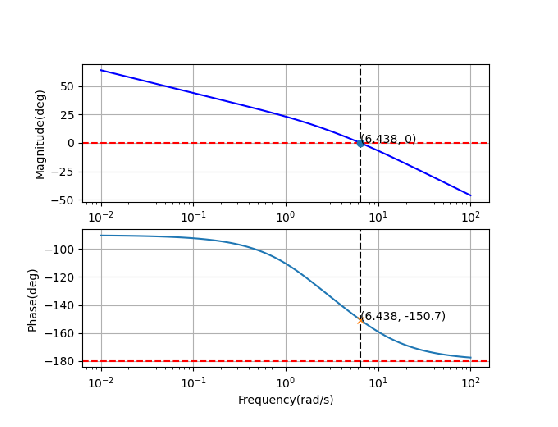
\includegraphics[width=\columnwidth]{./figs/ee18btech11031_2.eps}
  \caption{Graphs}
  \label{fig:ee18btech11031}
\end{figure}

The python code to obtain the graphs and results:

\begin{lstlisting}
codes/ee18btech11031.py
\end{lstlisting}

%\item 
{\em Gain} and {\em Phase} of Transfer Function 
\begin{align}
G\brak{j\omega} &= \frac{50\brak{j\omega+3}\brak{j\omega+5}}{j\omega\brak{j\omega+2}\brak{j\omega+4}\brak{j\omega+6}}
\end{align}
Gain:
\begin{align}
    \frac{100\sqrt{{\brak{\omega}^2+9}}\sqrt{\brak{\omega}^2+25}}{\omega\sqrt{\brak{\omega}^2+4}\sqrt{\brak{\omega}^2+16}\sqrt{\brak{\omega}^2+36}}
\label{eq:ee18btech11031_2}
\end{align}{}
Phase:
\begin{multline}
\tan^{-1} \brak{0}+\tan^{-1} \brak{\frac{\omega}{3}}+\tan^{-1} \brak{\frac{\omega}{5}}-\tan^{-1} \brak{\frac{\omega}{0}}\\-\tan^{-1} \brak{\frac{\omega}{2}} - \tan^{-1} \brak{\frac{\omega}{4}}-\tan^{-1} \brak{\frac{\omega}{6}} 
\label{eq:ee18btech11031_3}
\end{multline}
%\item Find the Phase Margin\brak {PM} and verify using the same code
\begin{align}
 PM = \angle G(j\omega_{gc}) + 180\degree \\
\omega_{gc}=\text{Gain Crossover Frequency}\\
\text{At }  \omega_{gc} \left| G\brak{s}\right|  = 1
\end{align}
\solution
\begin{align}
    \frac{100\sqrt{{\brak{\omega_{gc}}^2+9}}\sqrt{\brak{\omega_{gc}}^2+25}}{\omega{gc}\sqrt{\brak{\omega_{gc}}^2+4}\sqrt{\brak{\omega_{gc}}^2+16}\sqrt{\brak{\omega_{gc}}^2+36}} &= 1
\label{eq:ee18btech11031_4}
\end{align}
Solving Eq. \eqref{eq:ee18btech11031_4} {\em or} from Fig \ref{fig:ee18btech11031} :

\begin{align}
\implies
\omega_{gc} &= 6.438  \\
\angle G\brak{j\omega_{gc}} &= -150.725 \\
\implies
PM &= 29.275 
\end{align}

%\item Find the Gain Margin \brak{GM} and verify using the same code.
\begin{align}
 GM = 0 -G(j\omega_{pc}) db \\
\omega_{pc}=\text{Phase Crossover Frequency}
\end{align}
\begin{align}
\text{At }  \omega_{pc}, \angle G\brak{s}  = -180\degree
\label{eq:ee18btech11031_5}
\end{align}
% \\
%\solution
From Fig \ref{fig:ee18btech11031} ,we can say that phase  never crosses $-180\degree$ .
So , the gain margin is {\em infinite} and from the equation: \ref{eq:ee18btech11031_5}, $\omega_{pc}$ is non-existent.




%\end{enumerate}
